\section{Theorie}
Im vorliegenden Experiment wird eine LC-Kette, bestehend aus alternierenden Kapazitäten $C_1$ und $C_2$, genauer im Kapitel \ref{sec:Aufbau} beschrieben, untersucht werden.
Bevor die theoretischen Grundlagen dieser Schaltung erläutert werden, sollen zunächst grundlegendere Zusammenhänge erklärt werden, die für die weitere Erläuterungen vonnöten sind.
\label{sec:Theorie}
\subsection{Theoretische Grundlagen}
\subsubsection{Kirchhoffsche Regeln}
Um die Ströme und Spannungen in elektrischen Stromkreisen beschreiben zu können, werden die Kirchhoffschen Regeln genutzt.
Die erste Kirchhoffsche Regel, welche die Ströme beschreibt, ist die Knotenregel \eqref{eqn:knotenregel}.
Sie folgt unmittelbar aus der Ladungserhaltung und besagt, dass in jedem Knotenpunkt einer Schaltung die Summe aller eingehenden und ausgehenden Ströme verschwindet:
\begin{equation}
  \sum_{k=1}^n I_k = 0.
  \label{eqn:knotenregel}
\end{equation}
Die Spannungen werden durch die Maschenregel \eqref{eqn:maschenregel} beschrieben, welche die zweite Kirchhoffsche Regel darstellt.
Sie folgt aus dem Induktionsgesetz im Vakuum
\begin{equation}
\oint \vec{E} \cdot \vec{\symup{d}s} = 0
\end{equation}
und besagt, dass in jeder geschlossenen Masche der Schaltung die Summe der Spannungen null ergibt:
\begin{equation}
  \sum_{i=1}^n U_i = 0.
  \label{eqn:maschenregel}
\end{equation}
\subsubsection{Impedanzen bekannter elektrischer Bauelemente}
\label{sec:impedanzen}
Die Impedanzen eines ohmschen Widerstandes $R$, einer Induktivität $L$ sowie einer Kapazität $C$ sind gegeben durch
\begin{equation}
  Z_R = R,
\end{equation}
\begin{equation}
  Z_L = i \omega L
\end{equation}
sowie
\begin{equation}
  Z_C = \frac{-i}{\omega C}.
\end{equation}

\subsection{Dispersionsrelation einer LC-Kette}
Ein repräsentativer Ausschnitt der LC-Kette ist in Abbildung \ref{tfig:1} dargestellt.
\begin{figure}[H]
  \centering
  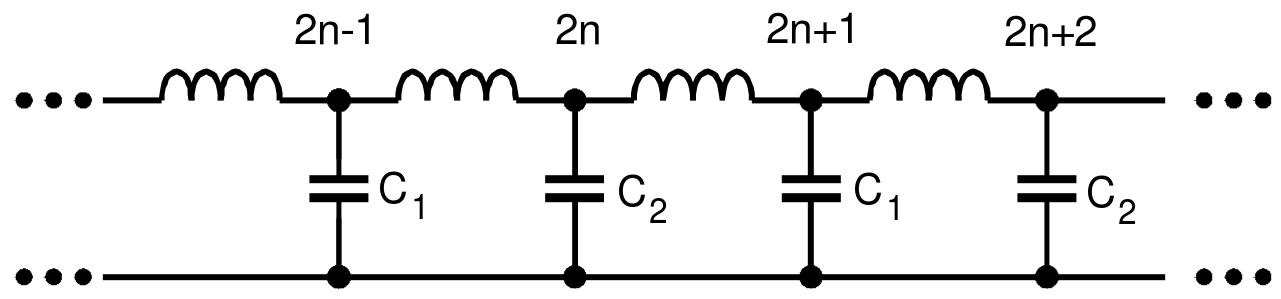
\includegraphics[height=3cm]{theorie_1.png}
  \caption{Schematischer Ausschnitt einer LC-Kette.}
  \label{tfig:1}
\end{figure}
Nach Anwendung der Knotenregel \eqref{eqn:knotenregel} sowie der Maschenregel \eqref{eqn:maschenregel} und unter Berücksichtigung der in Abschnitt \ref{sec:impedanzen} angegebenen Zusammenhänge folgen die beiden gekoppelten Gleichungen
\begin{align}
  \label{eqn:dif1}
  \frac{1}{L} \Bigl( -U_{2n} + 2 U_{2n+1} - U_{2n+2} \Bigr) - \omega^2 C_1 U_{2n+1} &= 0 \\
  \label{eqn:dif2}
  \frac{1}{L} \Bigl( -U_{2n-1} + 2 U_{2n+1} - U_{2n+1} \Bigr) - \omega^2 C_2 U_{2n} &= 0
\end{align}
für die LC-Kette.
Dabei bezeichnet $U_k$ jeweils die am zum $k$-ten Knotenpunkt gehörenden Kondensator anliegenden Spannung.
Als Lösungen für diese Gleichungen werden die Ansätze
\begin{align}
  \label{eqn:l1}
U_{2n+1} &= U_{0,1} \, \mathrm{e}^{i \theta (2n+1)} \, \mathrm{e}^{ i \omega t} \\
  \label{eqn:l2}
U_{2n} &= U_{0,2} \, \mathrm{e}^{i \theta (2n)} \, \mathrm{e}^{ i \omega t}
\end{align}
verwendet.
Hierbei bezeichnet $\theta$ die Phasenänderung pro Kettenglied sowie $\omega$ die Kreisfrequenz der Schwingung.
Durch Einsetzen von \eqref{eqn:l1} in \eqref{eqn:dif1} sowie \eqref{eqn:l2} in \eqref{eqn:dif2} erhält man durch Umformungen und Anwendung der Eulerformel die Beziehungen
\begin{align}
U_{0,1} \Bigl( \frac{2}{L} - \omega^2 C_1  \Bigr) - U_{0,2} \frac{2 \cos (\theta)}{L} &= 0, \\
-U_{0,1} \frac{2 \cos (\theta)}{L} - \omega^2 C_1 + U_{0,2} \Bigl( \frac{2}{L} - \omega^2 C_2  \Bigr)  &= 0.
\end{align}
Dieses Gleichungssystem lässt sich schreiben als
\begin{align*}
  \vec{U} \symbf{M} = 0
\end{align*}
mit der Matrix
\begin{equation}
  \symbf{M} =
  \begin{pmatrix*}[l]
    \frac{2}{L} - \omega^2 C_1 & -\frac{2}{L} \cos{(\theta)} \\
    -\frac{2}{L} \cos{(\theta)} & \frac{2}{L} - \omega^2 C_2
  \end{pmatrix*}.
\end{equation}
Nur für $\symup{det}(\symbf{M})=0$ ergeben sich nicht-triviale Lösungen dieses Gleichungssystems.
Hieraus folgt sofort die Dispersionsrelation zu
\begin{equation}
  \label{eqn:dispersion}
  \omega_{1/2}^2 = \frac{1}{L} \Bigl( \frac{1}{C_1} + \frac{1}{C_2} \Bigr) \pm \frac{1}{L} \sqrt{ \Bigl( \frac{1}{C_1} + \frac{1}{C_2} \Bigr)^2 - \frac{4 \sin^2 \! {\left(\theta \right)}}{C_1 C_2} }.
\end{equation}
Sie beschreibt das Verhältnis der Phasenänderung pro Kettenglied $\theta$ und der Kreisfrequenz $\omega$.
Die Dispersionskurve wird in Abbildung \ref{tfig:2} schematisch dargestellt.
\begin{figure}[H]
  \centering
  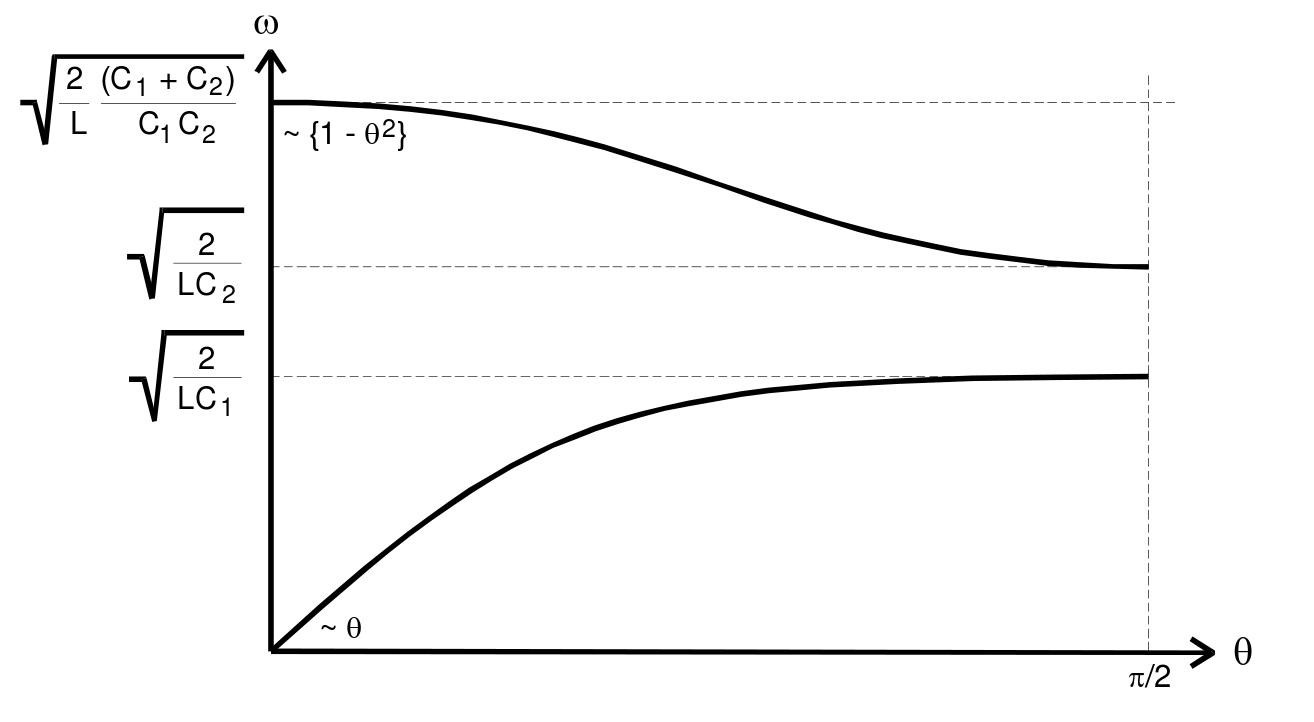
\includegraphics[height=8cm]{dispersionskurve.png}
  \caption{Kurve der Dispersionsrelation einer LC-Kette mit alternierenden Kapazitäten.}
  \label{tfig:2}
\end{figure}
Es fällt auf, dass sich die Kurve in zwei Äste aufteilt, von denen der obere Ast in Analogie zur Kristallphysik als optischer Ast, der untere als akustischer Ast bezeichnet wird.
Zudem ergibt sich ein Frequenzbereich
\begin{align*}
  \sqrt{\frac{2}{LC_1}} < \omega < \sqrt{\frac{2}{LC_2}},
\end{align*}
in dem Schwingungen nicht erzeugt werden können.
\subsection{Ausbreitungsgeschwindigkeit der Wellen}
Die Lösungen für die Spannungen $U_n$ besitzen die, in \eqref{eqn:l1} und \eqref{eqn:l2} spezifizierte, allgemeine Form
\begin{equation}
  \label{eqn:a1}
  U_k = U_0 \mathrm{e}^{i(\omega t - k \theta)}.
\end{equation}
Im Allgemeinen beschreibt die Phasengeschwindigkeit $v_{\text{Ph}}$ nun, mit welcher Geschwindigkeit sich Orte gleicher Phase in einer Welle ausbreiten:
\begin{equation}
  v_{\text{Ph}} = \frac{\increment{n}}{\increment{t}}.
\end{equation}
Betrachtet man nun jene Geschwindigkeit für die in \eqref{eqn:a1} angegebene Formel, ergibt sich eine Phasengeschwindgkeit von
\begin{equation}
    \label{eqn:phase}
  v_{\text{Ph}} = \frac{\omega}{\theta}.
\end{equation}
Für die Signalübertragung notwendig sind jedoch sogenannte Wellengruppen, welche durch eine sich fortpflanzende, einhüllende Funktion mit Anfang und Ende gekennzeichnet sind.
Schematisch ist eine solche Wellengruppe in Abbilidung \ref{tfig:3} dargestellt.
\begin{figure}[H]
  \centering
  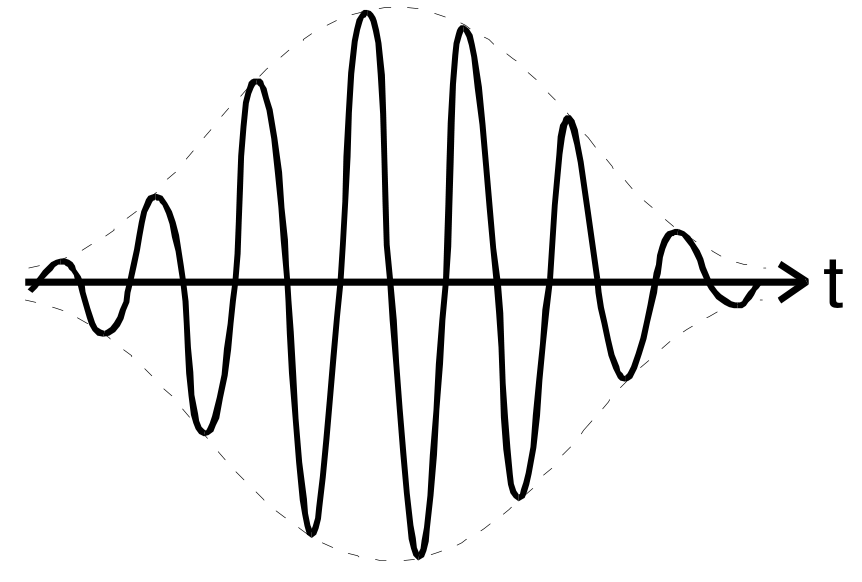
\includegraphics[height=5cm]{wellenpaket.png}
  \caption{Schematische Darstellung eines Wellenpaketes.}
  \label{tfig:3}
\end{figure}
Die Ausbreitung des Maximum dieses Wellenpaketes, welches aus mehreren Wellen mit verschiedenen Frequenzen und somit unterschiedlichen Phasengeschwindigkeiten besteht, wird als Gruppengeschwindigkeit $v_{\text{gr}}$ bezeichnet.
Um diese zu beschreiben, werde eine Welle mit der zeitabhängigen Amplitude
\begin{align*}
A(t) = A_0 \cos{(\omega t - \theta)}
\end{align*}
sowie eine mit der Amplitude
\begin{align*}
A'(t) = A_0 \cos{(\omega' t - \theta')}
\end{align*}
betrachtet, wobei sich die Frequenzen $\omega$ und $\omega'$ nur leicht unterscheiden sollen.
Nach Anwendung der Additionstheoreme sowie der Näherungen
\begin{align*}
  \frac{1}{2}(\omega + \omega') \approx \omega
\end{align*}
und
\begin{align*}
  \frac{1}{2}(\theta + \theta') \approx \theta
\end{align*}
ergibt sich
\begin{equation}
A(t) + A'(t) = 2 A_0 \cos{(\omega t - \theta)} \cos{(\frac{1}{2} (\omega - \omega')t - (\theta - \theta'))}.
\end{equation}
Dieses Phänomen, bei dem eine Welle mit Überlagerungsfrequenz durch eine einhüllende Welle mit Resonanzfrequenz entsteht, bezeichnet man als Schwebung.
Die Gruppengeschindigkeit $v_{\text{gr}}$ entspricht nun der Ausbreitungsgeschwindigkeit eines Schwebungsmaximas.
Dieses ergibt sich somit zu
\begin{equation}
  \label{eqn:gruppe}
  v_{\text{gr}} = \frac{\omega - \omega'}{\theta - \theta'} \: \stackrel{\stackrel{\omega \to \omega'}{\theta \to \theta'}}{=} \: \frac{\symup{d}\omega}{\symup{d}\theta}.
\end{equation}
Angewendet auf die in Formel \ref{eqn:dispersion} gefundene Dispersionsrelation für die alternierende LC-Kette ergibt sich
\begin{equation}
  v_{\text{Ph}} = \frac{\omega}{\arcsin{\Bigl( \frac{1}{2} L \omega^2 (C_1 + C_2) - \frac{1}{4} L^2 \omega^4 C_1 C_2   \Bigr)}}
\end{equation}
als Phasengeschwindigkeit sowie nach kurzer Rechnung auch die Gruppengeschwingkeit.
Diese Rechnung sei dem aufmerksamen Leser als Übung überlassen.
